\section{Easy Example}

In this section, we will go through an easy numerical example of the HHL algorithm.
The quantum circuit that we will be using contains 4 qubits.
The scheme of the quantum circuit is shown Fig. 2.
Firstly, we will have to set some preliminary values to make our calculations easier. 
Then, we will go through all 5 phases of the HHL algorithm \cite{qiskit_hhl}. 

\subsection{Preliminaries}
We are given the following matrix $A$ and the vector $\vec{b}$ 
\begin{equation}
   A = \begin{pmatrix} 1 & -\frac{1}{3}\\ -\frac{1}{3} & 1\\ \end{pmatrix}
\end{equation}

\begin{equation}
    \vec{b} = \begin{pmatrix} 0 \\ 1\\ \end{pmatrix}
\end{equation}

If we calculate the solution classically we will obtain the solution vector 
\begin{equation}
\vec{x} = \begin{pmatrix} \frac{3}{8}\\ \frac{9}{8}\\ \end{pmatrix}
\end{equation}

The HHL algorithm doesn't solve for the whole solution vector $\vec{x}$, as we are only interested in some estimation value $\bra x M \ket x$.
To compare the results of both methods we will take the probability ratio of the entries of our solution vector $\vec x$ and $\ket x$.
To calculate the probability ratio, we have to divide by the square of each entry of $\vec{x}$.
Thus, we obtain a ratio of
\begin{equation}
    \frac{ |x_0|^2}{ |x_1|^2}= \frac{\frac{9}{64}}{\frac{81}{64}} = \frac{1}{9}
\end{equation}
where $x_0$ and $x_1$ are the entries of $\vec x$.

To make our calculations, we will cheat by determining the eigenvectors and eigenvalues beforehand.
Normally, the QPE would calculate these numbers, but as the main focus of this paper is the HHL algorithm, we will not calculate the eigenvalues and eigenvector manually through QPE.
The eigenvectors of the matrix $A$ are
\begin{equation}
\vec{u_0} = \begin{pmatrix} \frac{-1}{\sqrt{2}}\\ \frac{-1}{\sqrt{2}}\\ \end{pmatrix}\\
\end{equation}

\begin{equation}
\vec{u_1} = \begin{pmatrix} \frac{-1}{\sqrt{2}}\\ \frac{1}{\sqrt{2}}\\ \end{pmatrix}
\end{equation}

These can be represented through amplitude encoding in our quantum circuit
\begin{equation}
\ket{u_0} = \frac{-1}{\sqrt{2}}\ket{0} + \frac{-1}{\sqrt{2}}\ket{1}
\end{equation}

\begin{equation}
\ket{u_1}= \frac{-1}{\sqrt{2}}\ket{0} + \frac{1}{\sqrt{2}}\ket{1} 
\end{equation}

Additionally, we also have to determine the eigenvalues. The eigenvalues $\lambda_j$ of the matrix $A$ are
\begin{equation}
\lambda_0 = \frac{2}{3}
\end{equation}

\begin{equation}
\lambda_1 = \frac{4}{3}
\end{equation}

We then have to encode the eigenvalues into a quantum state $\ket{\widetilde{\lambda_j}}$.
In the encoding scheme $\widetilde{\lambda_j} = N_q\lambda_jt/2\pi)$, we can freely choose a $t$ such that we obtain an easy encoding of the eigenvalues. 
Here $N_q$ refers to the number of qubits in our system, which means $N_q = 4$.
If we choose $t = 3\pi/4$, then we will obtain
\begin{equation}
\widetilde{\lambda_0} =\frac{4*\frac{2}{3}*\frac{3\pi}{4}}{2 \pi} =\frac{4*2*3\pi}{3*4* 2 \pi} = 1
\end{equation}
\begin{equation}
\widetilde{\lambda_1} =\frac{4*\frac{4}{3}*\frac{3\pi}{4}}{2 \pi} =\frac{4*4*3\pi}{3*4* 2 \pi} = 2
\end{equation}
which can be encoded through basis encoding into the quantum circuit.
Thus, we are left with these states
\begin{equation}
\ket{\widetilde{\lambda_0}} = \ket{01}
\end{equation}
\begin{equation}
\ket{\widetilde{\lambda_1}} = \ket{10}
\end{equation}

Now we can start with our procedure.

\subsection{Numerical walkthrough}

In Fig.~\ref{ex_circ_numerical} we can see that we have 1 qubit each for the a-register and b-register, corresponding to the ancilla bit and the input $\vec b$.
The c-register has 2 qubits, as we have to store the two eigenvalues $\lambda_1$, $\lambda_2$ we calculated just now.
Our starting state looks like this
\begin{equation}
\ket{\Psi_0} = \ket{0}_b\ \ket{00}_c\ \ket{0}_a = \ket{0000}
\end{equation}
all registers being initalized with the zero state.


\begin{figure}
    \centering
    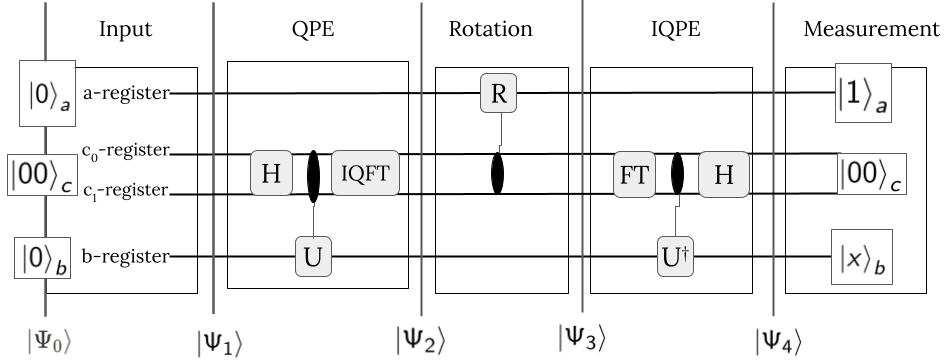
\includegraphics[width=8.5cm]{img/example_circuit_4_qubit_cropped.png}
    \caption{4-Qubit Circuit}
    \label{ex_circ_numerical}
\end{figure}


\subsubsection{State preparation}
    Here we have to encode our vector $\vec{b}$ into the quantum state $\ket{b}$, using amplitude encoding.
    We obtain
    \begin{equation}
    \vec{b} = \begin{pmatrix} 0\\ 1\\ \end{pmatrix}
    \Leftrightarrow \ket{b} = 0 \ket{0} + 1 \ket{1} = \ket{1} 
    \end{equation}
    which makes sense as the $\ket 1$ state is defined as the $\begin{pmatrix} 0\\ 1\\ \end{pmatrix}$ vector.
    After loading $\ket b$ into our quantum circuit, the state of the circuit is 
    \begin{equation}
    \ket{\Psi_1} = \ket{1}_b\ \ket{00}_c\ \ket{0}_a = \ket{1000}
    \end{equation}

\subsubsection{Quantum Phase Estimation}
    The QPE determines the eigenvalues $\lambda_j$ of the $A$ matrix. 
    These are stored in the c-register. 
    The b-register now stores $\ket b$ in the eigenbasis state of $A$ leading us to the following state
    \begin{equation}
    \ket{\Psi_2} = \ket{b}_b \ket{\widetilde{\lambda}}_c\ket{0}_a
    \end{equation}
    \begin{equation}
    \ket{\Psi_2} =\left(-\frac{1}{\sqrt{2}} \ket{u_0}_b \ket{01}_c +\frac{1}{\sqrt{2}} \ket{u_1}_b \ket{10}_c \right)  \ket{0}_a
    \end{equation}


\subsubsection{Inversion of the eigenvalues}
    Now we have to invert the eigenvalues. 
    This is achieved by rotating the a-registers by the eigenvalues in the c-register.
    This leaves us in this state

    \begin{equation}
     \begin{split}
    \ket{\Psi_3} =& \sum_{j=0}^{2^{1}-1} b_j \ket{u_j} \ket{\widetilde{\lambda}_j} \left(\sqrt{1-\frac{C^2}{\widetilde{\lambda}_j^2}}\ket{0} + \frac{C}{\widetilde{\lambda}_j} \ket{1}\right) \\
    =&-\frac{1}{\sqrt{2}} \ket{u_0} \ket{01}\left(\sqrt{1-\frac{1}{1^2}}\ket{0} + \frac{1}{1} \ket{1}\right) \\
    &+\frac{1}{\sqrt{2}}  \ket{u_1} \ket{10} \left(\sqrt{1-\frac{1}{2^2}}\ket{0} + \frac{1}{2} \ket{1}\right)
     \end{split}
    \end{equation}

    The ancilla bit is in a superposition and can either collapse to $\ket 0$ or $\ket 1$.
    We assume that our rotation was successful and we measure $\ket{1}$ in the ancilla qubit, then

    \begin{equation}
    \begin{split}
    \ket{\Psi_3} &=\sqrt{\frac{8}{5}}\left(\frac {1} {\widetilde{\lambda_0}} *-\frac{1}{\sqrt{2}} \ket{u_0}_b\ket{01}_c +\frac{1}{\widetilde{\lambda_1}}*\frac{1}{\sqrt{2}} \ket{u_1}_b\ket{10}_c\right)\ket{1}_a \\
    &=\sqrt{\frac{8}{5}}\left(-\frac{1}{\sqrt{2}} \ket{u_0}_b\ket{01}_c +\frac{1}{2\sqrt{2}} \ket{u_1}_b\ket{10}_c\right)\ket{1}_a 
    \end{split}
    \end{equation}

    Note that the b-register and c-register are entangled. We have to unentangle the registers.

\subsection{Inverse Quantum Phase Estimation}
    We now backtrack all the steps in the QPE through IQPE.
    The c-register is reset to the zero state again and the b-register contains our solution state $\ket x$.
    The state of the circuit looks like this
    \begin{equation}
    \ket{\Psi_4}= \ket{x}_b \ket{00}_c \ket{1}_a 
    \end{equation}
    \begin{equation}
    \ket{\Psi_4}=\frac{1}{2}\sqrt{\frac{2}{5}}  \left(\ket{0} +3 \ket{1} \right) \ket{00}_b \ket{1}_a
    \end{equation}

\subsection{Measurement}
    Now we have to measure the solution state $\ket x$.
    In the beginning, we decided to take the probability ratio as our solution. 
    To get the probability of $\ket{u_0}$ and $\ket{u_1}$ we have to square their coefficients
\begin{equation}
\begin{split}
c_0&=\left|\frac{1}{2}\sqrt{\frac{2}{5}}*1\right|^2 = \frac{1}{20}\\
c_1&=\left|\frac{1}{2}\sqrt{\frac{2}{5}}*3\right|^2 = \frac{9}{20}
\end{split}
\end{equation}

As expected our ratio is 
\begin{equation}
 \frac{\frac{1}{20}}{ \frac{9}{20} } = \frac 1 9
\end{equation}

